\chapter{Introduction}\label{chapter:introduction}

\section{Explosion of biomedical data}

In recent times, there has been a phenomenal rise in the amount of information available in the world. Since scientific articles remains the preferred way of publishing scientific research, there also has been a huge increase in the amount of scientific literature, particularly in the area of biomedical sciences. Pubmed \cite{pubmed}, the database of biomedical articles, boasts of more than 24 million scientific articles and is growing rapidly. In 2014 alone, PubMed have added more than a million articles. Figure \ref{fig:PubMedTimeLine} shows the growth of PubMed database in recent years.

\section{Need for automatic extraction of information}

With huge amount of information available in the biomedical literature, it has become impossible for researchers to keep track of all the developments in the field. Given the textual nature of this scientific literature, text-mining techniques are helping the researchers to extract relevant information from this gold mine without having to read each and every article. As a result, there has been tremendous increase in research in the area of text-mining biomedical literature. These techniques are intended to help researchers who cannot manually scavenge thousands of articles for information.

\begin{figure}
\centering
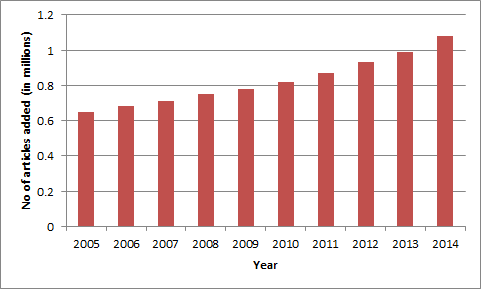
\includegraphics[scale=0.4]{figures/PubMedTimeLine.png}
\caption{Growth of PubMed in recent years}\label{fig:PubMedTimeLine}
\end{figure}

% TODO: 
\subsection*{Need for biomedical research community}
% 1. Write about why scientists both in biomedical and text-mining domain needs automatic information extractors. Need inputs on how this information

"Biomedical research" is an umbrella term used for research in various disciplines like biochemistry, immunology, microbiology, cytology, etc. To give an example, some of the problems studied in the area of biochemistry are protein-protein interaction, protein-ligand interaction, protein-subcellular localization, etc. All of these different biochemical processes play a vital role in proper functioning of the body and any impairment in these processes can have far reaching effect on human health, usually blowing into a full-fledged disease. It is no wonder that many researchers across the globe are working simultaneously on some of these problems and therefore, it becomes essential for such researchers to keep track of the recent advances and start building from there. 

Conventionally, the best method to keep oneself updated about recent scientific advances is by reading the scientific literature. This remains to be the best way in some areas of science where the scientific throughput is less and harder to achieve. However in some fields like biomedical sciences, due to huge volume of scientific literature, it has become very difficult for a researcher to stay updated about recent work being done in his area of interest. As pointed out by Cohen et.al. in \cite{cohen2005survey}, the knowledge discovery requires extracting information from research articles and there is no individual in a position to go through the extraordinarily large volume of information.

Therefore, the text-mining methods have a large role to play in assisting researchers to extract relevant information from the information trove, although with certain degree of confidence.

\section{Subcellular localization of Proteins}

% Explain about why do we need to know about subcellular localization of proteins
The subcellular localization of proteins is one of the most studied biochemical processes. The proteins play an important role in the functioning of cell machinery and are therefore called "building blocks of life". The creation of proteins consists of two main phases, viz. transcription and translation. The proteins are created in the cytoplasm by flow of genetic information from DNA (Deoxyribonucleic acid) to RNA (Ribonucleic acid) and from RNA to Proteins. The genetic information present in the DNA is converted to RNA by a process known as transcription. Transcription takes place in the nucleus of the cell. The RNA strand so created travels from nucleus to cytoplasm through the nuclear pores. In the cytoplasm, RNA strand is used to create a protein with the help of cellular machinery called as ribosomes. The process of converting RNA to a chain of amino acids called proteins is called translation. 

Although the proteins are created in the cytoplasm, they do not necessarily perform their biological functions in the cytoplasm. A protein can perform its function anywhere in the cell (cytoplasm or cellular organelle) or outside the  cell. Therefore, the biological function of the proteins largely depend on their location and knowledge of the subcellular location of the protein is key to understanding its biological function. The subcellular location is a generic term used to indicate the location, even if the protein exits from cell and perform its  function outside the cell.

\subsection*{Important role in drug research}
% 2. How automatic extraction of information will help in drug research

The proteins play a very important role in proper functioning of cell machinery and hence, an abnormality in their functioning can result in adverse effects, even leading to a disease. The study of proteins and their subcellular location is an important stage in the development of a drug. Drug researchers study the subcellular location of proteins which can help them identify suitable drug, vaccine or diagnostic treatment \cite{liu2007exploiting}. 


\subsection*{Current sources of information}
% Explain about 
%- Uniprot, Swissprot and Trembl. 
%- Also talk about the procedure followed by PubMed annotators and how locations are mentioned for each protein
%- Can also talk about sources where you can extract protein-location relation

Currently, the important sources of information about subcellular location of proteins are knowledge bases like UniProtKB \cite{magrane2011uniprot}, manual curation from the literature, high-throughput microscopy-based screens and prediction from primary sequence.

\subsection*{Need of automatic extraction}

Although the knowledge bases like UniProtKB \cite{magrane2011uniprot} has considerable amount of information about proteins, including their subcellular location, it is not complete and can be supplemented \cite{goldberg2015linked}. UniProtKB consists of two sections, viz. Swiss-Prot and TrEMBL. TrEMBL contains automatically annotated information about a protein whereas Swiss-Prot contains the information which is manually reviewed by a curator. Every curator is in charge of certain proteins and he/she extracts the information manually by reading the literature. Obviously, this process is cumbersome and time-consuming. In addition, owing to the large amount of articles being published daily, it is impossible for these curators to update the information in the database constantly. This often results in some lag between the information present in knowledge bases and information in most recent literature.

Automatic text-mining methods can help the manual curators as well as the researchers to keep them updated about the information that is not present in knowledge bases. The extraction of information about subcellular locations of proteins can also help experimental biologists to verify this information experimentally. The information might also be useful to predict the location of other proteins which have considerable sequence similarity with the protein whose information is extracted by text-mining.

I have developed a method to extract the subcellular locations of proteins, automatically from the literature using text-mining techniques. This involves extracting the semantic relationship between the entities, protein and subcellular location present in the text. Hence, this process is also called as relationship extraction. Henceforth, the relationship between protein and subcellular location will be shortened as protein-location throughout the rest of this document.

Section \ref{sec:existingWork} describes the related work done in this area. Chapter \ref{chapter:corpus} describes the process of data set annotation and the insights obtained during manual annotation. Chapter \ref{chapter:theory} explains the theoretical background of the methods described in chapter \ref{chapter:methods}. The results of the method are explained in chapter \ref{chapter:results}.

\section{Existing related work}\label{sec:existingWork}

There hasn't been so much of work done in the area of protein-subcellular localization relation extraction. There has been some projects which have tried to work on the same problem and there are a lot other projects that are working on an allied problem. This section presents an overview of the recent work done in the related area.


%Literature Survey
\subsection*{Using rich syntactic information for relation extraction - Liu.et.al}

Lie et.al [CITE:LIU] proposed a method for extraction of protein-organism (PO) relations and protein-location (PL) relations from the text using sytanctic parse trees. The protein-organism (PO) and protein-location (PL) relations are then merged to predict a ternary protein-organism-location (POL) relation.

The corpus used in this method is composed of MEDLINE titles and abstracts annotated by domain expert biologists and parsed by Charniak-Johnson parser.

The focus of this work is to extract relations present in the same sentence and does not considers the inter-sentence relations. Two models are developed for extraction of relations viz. Semantic Role Labeling based relation extraction (SRL) and Tree kernel based relation extraction (TRK). Both models use features extracted from syntactic parse trees.

The model based on SRL uses manually extracted features from syntactic parse trees. These features are extracted along the path from protein to location/organism. This model is then trained by a Binary SVM using default linear kernel from Joachim’s SVM light [CITE:JOACHIM SVMLIGHT].

The model TRK uses entire parse tree as input for tree kernel. The model is trained by default tree kernel from Moschetti’s SVM-light-TK-1.2 [CITE:MOSCHETTI'S TK].

\begin{figure}[hbtp]
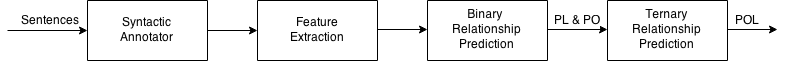
\includegraphics[scale=1]{figures/Liu_Flow.png}
\caption{Flow of information in relation extraction models }\label{fig:Liu}
\end{figure}


\begin{table}
\centering
\begin{tabular}{|l|l|l|l|l|}
\hline
\textbf{Relation} & \textbf{Precision} & \textbf{Recall} & \textbf{Fscore} & \textbf{Accuracy} \\ \hline
\textbf{PL} & 74.9 & 79.4 & 77.1 & 72.8 \\
PO & 73.9 & 78.1 & 75.9 & 72.6 \\
POL & 75.3 & 74.5 & 74.9 &  71.8\\ \hline
\end{tabular}
\caption{Results of SRL+TRK}\label{tab:Liu}
\end{table}

Table \ref{tab:Liu} shows the results for combination of both models.

\subsection*{BioNLP shared task and localization events}
% Explain what BioNLP event is and how localization is one of the 9 events that are meant to be extracted automatically
The BioNLP shared task [CITE:BIONLP SHARED EVENT] events in 2009 and 2011 focused on the aspects of event extraction from Biomedical literature. The BioNLP events provided an annotated corpus to the the text-mining community and asked for submission of innovative solutions for the tasks. One of the tasks was shared task in which the events present in the text have to be extracted. The data for shared task was a subset of GENIA event corpus [CITE:Genia event corpus]. Although, the original GENIA event corpus consists of 35 events, the shared task event corpus consisted of 9 events. One of the events common to both BioNLP event corpus as well as the main GENIA event corpus is localization event and therefore, the methods employed in these BioNLP events can be an important resource of study for the purpose of protein-subcellular location extraction.

\subsubsection*{Some of the issues with BioNLP corpus}

Although localization task is quite similar to protein-subcellular location extraction task, there are subtle differences which disallows using the same methods as it is for our task of protein-subcellular location extraction. 

One of the issues is that not all the locations found in the GENIA event corpus are subcellular locations. Some of them are even specific cells or tissues in the body. Some localization events were annotated without any mention of actual location but with the presence of a clue which hints that the text contains a localization event. In addition, the location mention contains extraneous words that are a part of the phrase but not absolutely essential for location mention. Owing to all these problems, we decided not to use GENIA event corpus as it is, develop our own corpus and develop a method using it.

\subsubsection*{State of the art in BioNLP'09}
%Work of Björne et al

The method developed by Björne et.al. [CITE:BJORNE PAPER] registered the state of the art performance in BioNLP Shared Task Event 2009. 

The shared task of event extraction consisted of three stages viz. Trigger detection, argument detection and event extraction. Triggers are the tokens or set of tokens that indicate the presence of the event. Once the triggers are detected, the triggers can be joined to other triggers or proteins as a part of predicate-argument structures. Finally, the triggers and their arguments are suitable combined to form an event.

This method extract events from the same sentence and do not look for inter-sentence event. The method developed by Björne et.al. represents a sentence as a graph where nodes are the tokens of the sentence and dependency relations are the edges between them. Every entity (Protein/DNA/RNA) forms a node in the graph as well. The event triggers are recognized and they also form a node in the graph. The edge between the trigger and argument is classified mainly as theme, cause,  negation etc. The model is trained by rich set of features extracted from the graph. For every stage of event extraction, somewhat different set of features are used. 

The sentences are tokenized and parsed before processing. The task of event extraction is accomplished in 3 steps:

\begin{enumerate}
\item \textbf{Trigger Recognition}: Each token is passed into multi-class SVM which predicts the event class depending on feature set. Each event class recognized forms a node in the final graph.

\item \textbf{Argument/Edge detection}: Every edge between event-event nodes and event-entity nodes is classified into theme, cause or negation.

\item \textbf{Semantic post-processing}: It is a rule based step to remove irrelevant connections. 
\end{enumerate}

The method uses BioNLP event corpus as the dataset and Joachim's SVM Light [CITE: JOACHIM MULTICLASS] for multiclass classification. Different multiclass classifier are built for classifying triggers and edges between triggers and arguments.

Following are the results of the method developed by Björne et.al.:

\begin{table}[h]
\centering
\begin{tabular}{|l|l|l|l|l|}
\hline
\textbf{Event Class} & \textbf{\# Events} & \textbf{Recall} & \textbf{Precision} & \textbf{Fscore} \\ \hline
\textbf{Localization} & 174 & 49.43 & 81.90 & 61.65 \\
Total & 3182 & 46.73 & 58.48 & 51.95\\ \hline
\end{tabular}
\caption{Results of Graph based event processing}
\end{table}

\subsubsection*{Using MLN for event extraction (Yashikawa et.al)}

Extending the results of Björne et.al., Yashikawa et.al. [CITE:YASHIKAWA] used coreference resolution to extract relations that span over multiple sentences in 
addition to extracting relations from same sentence. 

Yashikawa et.al.uses GENIA event corpus instead of BioNLP'09 corpus since GENIA corpus provides proper cross-sentence coreference. They show that the SVM multiclass method proposed by Bj{\"o}rne et.al. gives better results if it makes use of coreference annotation. In addition, they also developed a new model based on joint Markov Logic Network (MLN) which improved the results significantly.

The property of transitivity is used such that if there is a relation between event trigger \& entity and the entity has antecedent which can be resolved through anaphora/coreference resolution, then there is a relation between event \& antecedent.

%TODO: Write in formulation

The MLN model achieves a F1 score of 53.8 with naive coreference resolver and 56.7 with gold coreference annotation. 

\subsubsection*{COMPARTMENTS}

%Write about compartments 
%- Imai K etal. compartment reference 19
%- BacelLo compartment reference 20

Binder et.al. [CITE:COMPARTMENT] designed the COMPARTMENTS resource which integrates protein-subcellular location relations from different sources such as databases and prediction tools. To create a uniform representation of the information, the proteins and localizations are mapped to common protein identifiers and GO Ontology terms. Confidence scores are assigned to the localization evidence to enable comparison of different types and sources of evidence. The unified location evidence for a protein is then visualized on a schematic cell to  provide a simple overview.

There are different channels or sources from which the information is collected. The first channel is a \textit{knowledge} channel which contributes information based on annotation from databases like UniProtKB, MGI, SGD, FlyBase and WormBase. The second channel of information called \textit{experiments} is based on HPA - ongoing effort to experimentally validate  the tissue expression and subcellular localization for entire set of human proteins. The third channel which is of particular interest to us is \textit{automatic text mining} and the fourth channel of information is \textit{predictions} which depend on prediction of subcellular location depending on protein sequence.

The automatic text mining channel contributes information extracted by a text-mining method. The text-mining method which extracts information from MEDLINE abstracts works on the fact that more the protein and cellular compartment are co-mentioned, the more likely the protein is localized to that compartment. This leads to calculation of a score that determines the probability/confidence of localization of a protein to a cellular compartment. This text-mining method can be useful for comparing the performance with our method.

\section{Need for a dedicated method}
%
%- Explain about how localization event extraction tasks differ from our task
%- Explain about how coreference resolution takes a lot of time and isn't really accurate
%- Explain how many of the PL relations can exist outside same sentence

As mentioned previously, the GENIA event corpus or the BIONLP shared task corpus cannot be directly used for extracting protein-subcellular location relations. Therefore, there is a need to have a dedicated corpus designed for the purpose of training the text-mining method.

In addition, using the nuances of the new corpus, the new method can be trained on the corpus annotated and can produce better results.

Although, the model developed by Yashikawa et.al. extracts relations spanning over multiple sentences, extracting coreference information from the text at run-time is pretty slow. The method of Yashikawa et.al could work since their intention was not to create a runtime relation extraction.

We had decided to develop a dedicated text-mining method to extract protein location relations present in the corpus. We did not focused just on the same sentence relations but also on difference sentence relations in which the participating entities are in different sentences. In our annotated corpus, we also found out that 40\% of total relations cross sentence boundaries and therefore, developing a method that would consider different sentence relations would help us to extract more relations from the data.




















%The relation between PROTEIN and LOCALIZATION tells about the location where the protein may lie. The location can be a subcellular location as well as it can be an extracellular location. The location of PROTEIN is closely associated with its biological function and an ability to predict its location will be helpful to identify suitable drug, vaccine and diagnostic treatment ~\parencite{liu2007exploiting}. \citep{liu2007exploiting}. The prediction of protein location can also be extrapolated to some proteins for which localization is not known but it holds structural similarity with proteins for which localization are known. Therefore, in context of natural language processing, the problem of relation extraction between a protein and localization can be put simply as: recognizing whether a "protein" lies in the "location" if the words "protein" and "location" are found in the biomedical text that is being processed.
%
%The key problem while developing text mining tools on biomedical texts is the availability of annotated corpus. However, the advent of GENIA corpus\citep{kim2003genia} have facilitated the development of text mining methods. With the availability of GENIA event corpus \citep{kim2008corpus} and introduction of BioNLP'09 shared task data\citep{kim2009overview}, research in the area of event extraction has intensified. One of the events addressed in the areas of event extraction is localization. However, localization event extraction techniques concentrate mainly on events that change the location of biological entities such as protein. They do not focus so much on the existing state of localization of protein. Therefore, the problem of relation extraction that we are trying to address is not similar to event extraction proposed in BioNLP'09 Shared Task.
%
%There has been some research in the areas of relation extraction with respect to protein localization \citep{liu2007exploiting}. However, they do not take into account cross sentence relations. There have also been some research as a sub problem addressed in event extraction techniques \citep{bjorne2009extracting} \citep{yoshikawa2011coreference}. However, they do not focus solely on relation extraction and have developed their method to be able to address event extraction as a whole. Therefore, there is need to develop a text mining approach which addresses the problem of relation extraction for protein localization while considering inter-sentence as well as intra-sentence relations.


%\section{Section}
%Citation test~\parencite{latex}.

%\subsection{Subsection}
%See~\autoref{fig:sample}.
%
%\begin{figure}[htsb]
%  \centering
%  
\includegraphics{logos/tum}
%  \caption[Example figure]{An example for a figure.}\label{fig:sample}
%\end{figure}
%
%\section{Section}
%
%See~\autoref{tab:sample}, \autoref{fig:sample-drawing}, \autoref{fig:sample-plot}, \autoref{fig:sample-listing}.
%
%\begin{table}[htsb]
%  \caption[Example table]{An example for a simple table.}\label{tab:sample}
%  \centering
%  \begin{tabular}{l l l l}
%    \toprule
%      A & B & C & D \\
%    \midrule
%      1 & 2 & 1 & 2 \\
%      2 & 3 & 2 & 3 \\
%    \bottomrule
%  \end{tabular}
%\end{table}
%
%\begin{figure}[htsb]
%  \centering
%  % This should probably go into a file in figures/
%  \begin{tikzpicture}[node distance=3cm]
%    \node (R0) {$R_1$};
%    \node (R1) [right of=R0] {$R_2$};
%    \node (R2) [below of=R1] {$R_4$};
%    \node (R3) [below of=R0] {$R_3$};
%    \node (R4) [right of=R1] {$R_5$};
%
%    \path[every node]
%      (R0) edge (R1)
%      (R0) edge (R3)
%      (R3) edge (R2)
%      (R2) edge (R1)
%      (R1) edge (R4);
%  \end{tikzpicture}
%  \caption[Example drawing]{An example for a simple drawing.}\label{fig:sample-drawing}
%\end{figure}
%
%\begin{figure}[htsb]
%  \centering
%
%  \pgfplotstableset{col sep=&, row sep=\\}
%  % This should probably go into a file in data/
%  \pgfplotstableread{
%    a & b    \\
%    1 & 1000 \\
%    2 & 1500 \\
%    3 & 1600 \\
%  }\exampleA
%  \pgfplotstableread{
%    a & b    \\
%    1 & 1200 \\
%    2 & 800 \\
%    3 & 1400 \\
%  }\exampleB
%  % This should probably go into a file in figures/
%  \begin{tikzpicture}
%    \begin{axis}[
%        ymin=0,
%        legend style={legend pos=south east},
%        grid,
%        thick,
%        ylabel=Y,
%        xlabel=X
%      ]
%      \addplot table[x=a, y=b]{\exampleA};
%      \addlegendentry{Example A};
%      \addplot table[x=a, y=b]{\exampleB};
%      \addlegendentry{Example B};
%    \end{axis}
%  \end{tikzpicture}
%  \caption[Example plot]{An example for a simple plot.}\label{fig:sample-plot}
%\end{figure}
%
%\begin{figure}[htsb]
%  \centering
%  \begin{tabular}{c}
%  \begin{lstlisting}[language=SQL]
%    SELECT * FROM tbl WHERE tbl.str = "str"
%  \end{lstlisting}
%  \end{tabular}
%  \caption[Example listing]{An example for a source code listing.}\label{fig:sample-listing}
%\end{figure}
